


\section{Analysis of semantic distance}
It is desirable to show that $S_{k}(T_{1},T_{2})$ is a metric. This is well known for $k=1$ \citep{deza2013}, but we wish to extend the proof to larger values of $k$.

In order to rove that $S_{k}(T_{1},T_{2})$ is a metric we first represent the terms associated with a set of sequences using a venn diagram (\Cref{fig:sdvenn}) where $p$, $q$, $s$, and $t$ each represent a mutually exclusive and collective exhaustive subsets of terms in $T_{1}$, (where any of these sets may be the empty set) , and similarly define $T_{2}=\{q, r, t, u\}$, we can rewrite \Cref{eq:semantic_distance} as

\[
S_{k}(T_{1},T_{2})=\left( \left[ \underset{t\in p \cup s}{\sum} ia(t) \right]^{k} + \left[ \underset{t\in r \cup u}{\sum} ia(t) \right]^{k} \right)^{1/k}
\]

In an abuse of notation where we simply refer to the sum of $ia$ values for terms in each set as the set itself, the above equation can be further simplified and written as

\[
S_{k}(T_{1},T_{2})=\left( \left[ p+s\right]^{k} + \left[ r+u\right]^{k} \right)^{1/k}
\]


%%%%%%%%%%%%%%%%%%%%%%
%%%%%%%%%%%%%%%%%%%%%%
\begin{figure*}[h!]
\begin{centering}
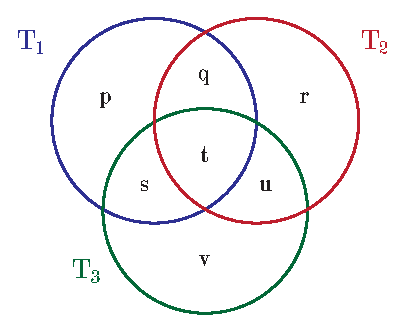
\includegraphics[width=0.45\linewidth]{Figures/sdproof/venn}
\par\end{centering}
\caption[A Venn diagram]{A Venn diagram showing the subsets of terms used to calculate the semantic distance between three pairs of annotations, $T_{1}$, $T_{2}$, and $T_{3}$. }
\label{fig:sdvenn}
\end{figure*}
%%%%%%%%%%%%%%%%%%%%%%
%%%%%%%%%%%%%%%%%%%%%%



\begin{theorem}
$S_{k}$ between two sets of terms, $T_{1}$ and $T_{2}$, is a metric for any real number $k \geq 1$.
\end{theorem}

\begin{proof}
%\begin{lemma}[Non-negativity]

~\begin{itemize}

\item \emph{Non-negativity}\\
The non-negativity of $S_{k}(T_{1},T_{2})$ is ensured by the fact that the information accretion, $ia(t)$, of an individual term is non-negative.  Because the conditional probability of a term given its parents, $\Pr (t|parents)$ is always $\geq 0$ and $\leq 1$, by virtue its information accretion, $-\log (t|parents)$, is always non-negative.
%\end{lemma}

%\begin{lemma}[Identity and indiscernibility]

\item \emph{Identity and indiscernibility}\\
$T_{1}=T_{2}$ if and only if $S_{k}(T_{1},T_{2})=0$.  First, if $T_{1}=T_{2}$, then $p, s, r, u = \varnothing$, and the resulting $ru(T_{1},T_{2})$, $mi(T_{1},T_{2})$, and $S_{k}(T_{1},T_{2})$ values will be zero.  Second, if $S_{k}(T_{1},T_{2})=0$ we know that $T_{1}=T_{2}$.  This is because the sum of information accretion values for any combination of terms will always be greater than zero, the only way that $ru(T_{1},T_{2})$ and $mi(T_{1},T_{2})$ can be equal to zero is when $p, s, r, u = \varnothing$.  When these sets are empty, it must be the case that $T_{1}=T_{2}$; and all terms in $T_{1}$ and $T_{2}$ are the same.
%\end{lemma}

%\begin{lemma}[Symmetry]
\item \emph{Symmetry}\\
$S_{k}(T_{1},T_{2})=S_{k}(T_{2},T_{1})$ because of the commutative property of addition, and the symmetric nature of $ru$ and $mi$.  For example, it can be shown that 
\[
ru(T_{1},T_{2}) = mi(T_{2},T_{1}),
\]
because $(p+s)=(p+s)$.
%\end{lemma}

%\begin{lemma}[Triangle inequality]
\item \emph{Triangle inequality}\\
Here we prove that $S_{k}(T_{1}, T_{2})+S_{k}(T_{1},T_{3}) \geq S_{k}(T_{2},T_{3})$ by showing that
\[
\left[\left(p+s\right)^{k}+\left(r+u\right)^{k}\right]^{\frac{1}{k}}+\left[\left(p+q\right)^{k}+\left(v+u\right)^{k}\right]^{\frac{1}{k}}\geq\left[\left(q+r\right)^{k}+\left(s+v\right)^{k}\right]^{\frac{1}{k}}
\]
where all elements are non-negative.
In order to prove this we rely on the Minkowski inequality, which can be expressed as

\[
 \left(\sum\limits_{i=1}^{n}  a_{i}^k \right)^{1/k} + \left(\sum\limits_{i=1}^{n}  b_{i}^k \right)^{1/k} \geq \left( \sum\limits_{i=1}^{n} \left[ a_{i} + b_{i} \right]^{k} \right)^{1/k}, 
\]

%The Minkowski inequality (which holds for $k\geq1$) is applied to theleft-hand side to obtain
where, for the sake of simplicity absolute value symbols have been omitted.  We first modify the left-hand side, using the Mikowski inequality,
\[
\left[\left(p+s\right)^{k}+\left(r+u\right)^{k}\right]^{\frac{1}{k}}+\left[\left(p+q\right)^{k}+\left(v+u\right)^{k}\right]^{\frac{1}{k}}\geq\left[\left(r+u+p+q\right)^{k} +  \left(p+s+v+u\right)^{k} \right]^{\frac{1}{k}},
\]
by setting the set $a = ( r+u , p+s )$ and $b = ( p+q, v+u )$.

Since we know that inequalities are transitive (i.e. if $a>b$ and $b>c$ then $a>c$), and it can be shown that

\[
\left[\left(r+u+p+q\right)^{k} +  \left(p+s+v+u\right)^{k} \right]^{\frac{1}{k}}\geq\left[\left(q+r\right)^{k}+\left(s+v\right)^{k}\right]^{\frac{1}{k}},
\]
the original formula has been proven.


%\end{lemma}
\end{itemize}
\end{proof}
